\documentclass[11pt,a4paper]{article}

\usepackage[a4paper,margin=2.3cm]{geometry}
\usepackage[T1]{fontenc}
\usepackage{textcomp}
\usepackage{graphicx}
\usepackage{amsmath}
\usepackage{amssymb}
\usepackage{booktabs}
\usepackage{tabularx}
\usepackage{siunitx}
\usepackage{caption}
\usepackage{subcaption}
\usepackage{float}
\usepackage{placeins}
\usepackage{xcolor}
\usepackage{microtype}
\usepackage{hyperref}
\usepackage{cleveref}
\usepackage{enumitem}
\usepackage{titlesec}
\setlist{itemsep=1pt,topsep=3pt,parsep=0pt}

\sisetup{detect-weight=true, detect-family=true}

\emergencystretch=3em
\sloppy
\titlespacing*{\section}{0pt}{10pt}{6pt}

\graphicspath{{generated_figures/july14_193548_422/}{../PresentationAssets/}}

\hypersetup{
  colorlinks=true,
  linkcolor=blue!50!black,
  citecolor=blue!50!black,
  urlcolor=blue!50!black,
  pdftitle={Multi-RCM Kinematic Control for a ROSA-like Surgical Robot in Unity},
  pdfauthor={Samuele Civale, Alexandru Vivian Pita, Francesca Forghieri}
}

\newcommand{\pass}{\textcolor{teal!60!black}{\textbf{PASS}}}
\newcommand{\fail}{\textcolor{red!70!black}{\textbf{FAIL}}}
\newcommand{\code}[1]{\texttt{#1}}

\title{\textbf{Multi-RCM Kinematic Control for a ROSA-like Surgical Robot}\\[2pt]
\large A Unity Simulation of Task-Space Remote-Center-of-Motion Control\\
with Target-Centred and Entry-Centred Operating Modes}

\author{
Samuele Civale -- 1938135 \\
Alexandru Vivian Pita -- 1948533 \\
Francesca Forghieri -- 2217594
}
\date{July 2026}

\begin{document}
\maketitle
\vspace{-8pt}

\begin{abstract}
\noindent This report documents a Unity-based simulation of a six-degree-of-freedom, ROSA-like manipulator regulating a needle-like tool under a \emph{Remote Center of Motion} (RCM) constraint. The controller is a from-scratch, purely kinematic damped-least-squares (DLS) scheme with a null-space secondary objective and an explicit penetration coordinate $\lambda$ along the tool shaft, in the spirit of Aghakhani et al.\ (ICRA 2013)~\cite{aghakhani2013}. Four modes are implemented: an entry-centred RCM with a fixed tip target, a target-centred RCM with a conical entry-side motion, a three-phase safe-insertion sequence, and an entry-centred RCM with a conical tip motion around a deep target. All quantitative results are computed from one selected continuous log (\texttt{project4\_multircm\_20260714\_193548\_422.csv}, 2696 samples, \SI{157.3}{\second}) that visits all four modes. Settled entry-RCM error stays sub-millimetre in every regulated task (max \SI{0.151}{\milli\meter} in safe insertion, \SI{0.834}{\milli\meter} in Task~4), and the final insertion tip-to-target error is \SI{0.467}{\milli\meter}, both comfortably inside the clinically motivated \SI{2}{\milli\meter}/\SI{3}{\milli\meter} thresholds. Conical-reference tracking is looser (Task~2: mean \SI{4.96}{\milli\meter} on an \SI{8.79}{\milli\meter} commanded radius; Task~4: mean \SI{3.19}{\milli\meter} on a \SI{13.8}{\milli\meter} radius), a direct consequence of pure-proportional feedback with no feedforward term. The implementation is compared aspect-by-aspect with the ICRA 2013 reference formulation, and functionality present in code but inactive in this run (skull-avoidance null-space term, Task-2 joint-4 active-set guard) is identified explicitly.
\end{abstract}

% =====================================================================
\section{Introduction and Motivation}
\label{sec:intro}
% =====================================================================

Stereotactic and minimally invasive neurosurgical procedures -- biopsy, electrode placement, needle insertion -- require a rigid tool to reach a deep target through a single, pre-planned entry point. Once fixed, any lateral motion of the tool shaft at that opening risks tissue damage along the surgical corridor. The \emph{Remote Center of Motion} (RCM) formalizes ``pass through this fixed point while pivoting freely otherwise'': a virtual pivot, external to the robot's own joints, through which the tool axis must pass while the tip performs a clinically meaningful motion elsewhere. Mechanical RCM devices enforce this passively; a \emph{software}/control-based RCM instead adds a velocity-level task to a general-purpose serial arm, trading mechanical simplicity for a dependence on accurate entry-point registration.

This project implements and evaluates an RCM-constrained kinematic controller in Unity for a procedurally generated, ROSA-like 6-DOF manipulator, built from scratch in C\# (no physics engine, no external IK library). It follows the idea introduced by Aghakhani et al.\ at ICRA~2013~\cite{aghakhani2013} of treating the RCM condition as an explicit penetration coordinate $\lambda$ solved together with the joint velocities. Four operating modes are implemented, corresponding to two placements of the effective RCM (entry point or target) and a three-phase safe-insertion sequence transitioning between them. The report (i) reconstructs the kinematic model and control logic directly from the C\# source, (ii) analyses the tracking and safety behaviour from one selected experimental log, and (iii) compares the approach, aspect by aspect, with the ICRA 2013 reference.

% =====================================================================
\section{Related Work}
\label{sec:related}
% =====================================================================

RCM realizations range from purely mechanical linkages to software-defined constraints solved as part of the inverse-kinematics problem; within the control-based family, RCM satisfaction has been obtained by extending the task Jacobian with an explicit RCM block, by real-time constrained optimization, or by formulating the RCM condition as an equality constraint on a point sliding along the tool shaft. This project follows the last family.

The reference paper is N.~Aghakhani, M.~Geravand, N.~Shahriari, M.~Vendittelli, G.~Oriolo, \emph{``Task Control with Remote Center of Motion Constraint for Minimally Invasive Robotic Surgery,''} ICRA 2013, pp.~5807--5812~\cite{aghakhani2013}. It expresses the RCM point $p_{\mathrm{RCM}}$ as a point sliding, with coordinate $\lambda\in[0,1]$, along the segment between two consecutive DH frame origins of the link passing through the trocar. Differentiating yields an RCM Jacobian $J_{\mathrm{RCM}}(q,\lambda)$ mapping $(\dot q,\dot\lambda)$ to $\dot p_{\mathrm{RCM}}$; imposing $\dot p_{\mathrm{RCM}}=0$ enforces the trocar condition as part of an \emph{extended task} $t_{\mathrm{EXT}}=(t,\,p_{\mathrm{trocar}}-p_{\mathrm{RCM}})$, solved by
$
(\dot q,\dot\lambda)^{\!\top} = J^{\#}\,\mathrm{diag}(K_t,K_{\mathrm{RCM}})\,e_t + (I-J^{\#}J)\,w,
$
with $J^{\#}$ the pseudoinverse of the extended Jacobian and $w$ a null-space vector regulating $\lambda$ toward a fixed nominal $\lambda_0$. The paper validates this on a simulated visual-servoing task (KUKA KR5, Webots) and a 9-DOF constrained-motion example (DLR MIRO); both are simulation studies. \Cref{sec:comparison} compares this formulation systematically with the present implementation.

% =====================================================================
\section{System and Robot Model}
\label{sec:architecture}
% =====================================================================

The project is a Unity scene built procedurally at runtime by \code{Project4SceneBuilder} (\code{Start()}): entry/target markers, an optional skull sphere, the robot and its controller, ground, lighting, and a keyboard-only free-fly camera. Every visual element is generated by the controller itself, so the DH table, gains, and task logic can be changed purely in C\# without touching the \code{.unity} file. In the scene used for the analysed log, \code{createSkull} is enabled (radius \SI{0.118}{\meter}); \cref{sec:discussion} clarifies what this sphere does and does not guarantee.

The manipulator is a procedurally generated 6-revolute-joint (6R) arm described by standard DH parameters (\cref{tab:dh}), documented in the source as a \emph{plausible ROSA-like} arm, not the manufacturer's real parameters. The tool is a rigid, non-actuated extension of length $L=\SI{0.283}{\meter}$ along the wrist $z$-axis (physical radius \SI{1.2}{\milli\meter}), adding the penetration coordinate $\lambda$ as a seventh controlled state, $x=(q,\lambda)\in\mathbb{R}^7$. The initial posture is $q_0=(0,5.24,-81.16,0,59.36,0)^{\circ}$.

\begin{table}[H]
\centering\small
\caption{Default DH parameters (\code{SetDefaultDH()}). $\theta_{\mathrm{offset}}=0$ for every link.}
\label{tab:dh}
\begin{tabular}{c S[table-format=1.3] S[table-format=-3.0] S[table-format=1.2] S[table-format=-3.0] S[table-format=3.0]}
\toprule
Link $i$ & {$a_i$ [m]} & {$\alpha_i$ [deg]} & {$d_i$ [m]} & {$q_{i,\min}$ [deg]} & {$q_{i,\max}$ [deg]} \\
\midrule
1 & 0.045 & -90 & 0.42 & -170 & 170 \\
2 & 0.420 &   0 & 0.00 & -120 & 120 \\
3 & 0.055 & -90 & 0.00 & -150 & 150 \\
4 & 0.000 &  90 & 0.36 & -170 & 170 \\
5 & 0.000 & -90 & 0.00 & -120 & 120 \\
6 & 0.000 &   0 & 0.12 & -360 & 360 \\
\bottomrule
\end{tabular}
\end{table}

\textbf{Software.} Four project-authored C\# scripts implement the simulation: \code{ROSADoubleRCMController.cs} (1656 lines -- kinematic model, control law, task/phase state machine, integration, visualization, CSV logging; the core deliverable), \code{Project4SceneBuilder.cs} (201 lines -- scene bootstrap), \code{FreeFlyCameraKeyboard.cs} (139 lines -- viewing aid only), and \code{RCMDiagnosticPlayerBuilder.cs} (28 lines -- editor-only headless-build utility). Offline analysis uses a Python script, \code{analyze\_rcm\_logs\_clean.py} (698 lines, unmodified), invoked by a thin report-only wrapper on exactly one CSV file. Every \SI{0.05}{\second} (\SI{20}{\hertz}) the controller logs tip/RCM/reference positions, all live error metrics, joint angles/velocities, $\lambda,\dot\lambda$, task/mode/phase labels, frame time/FPS, and pass/fail flags.

\begin{figure}[H]
\centering
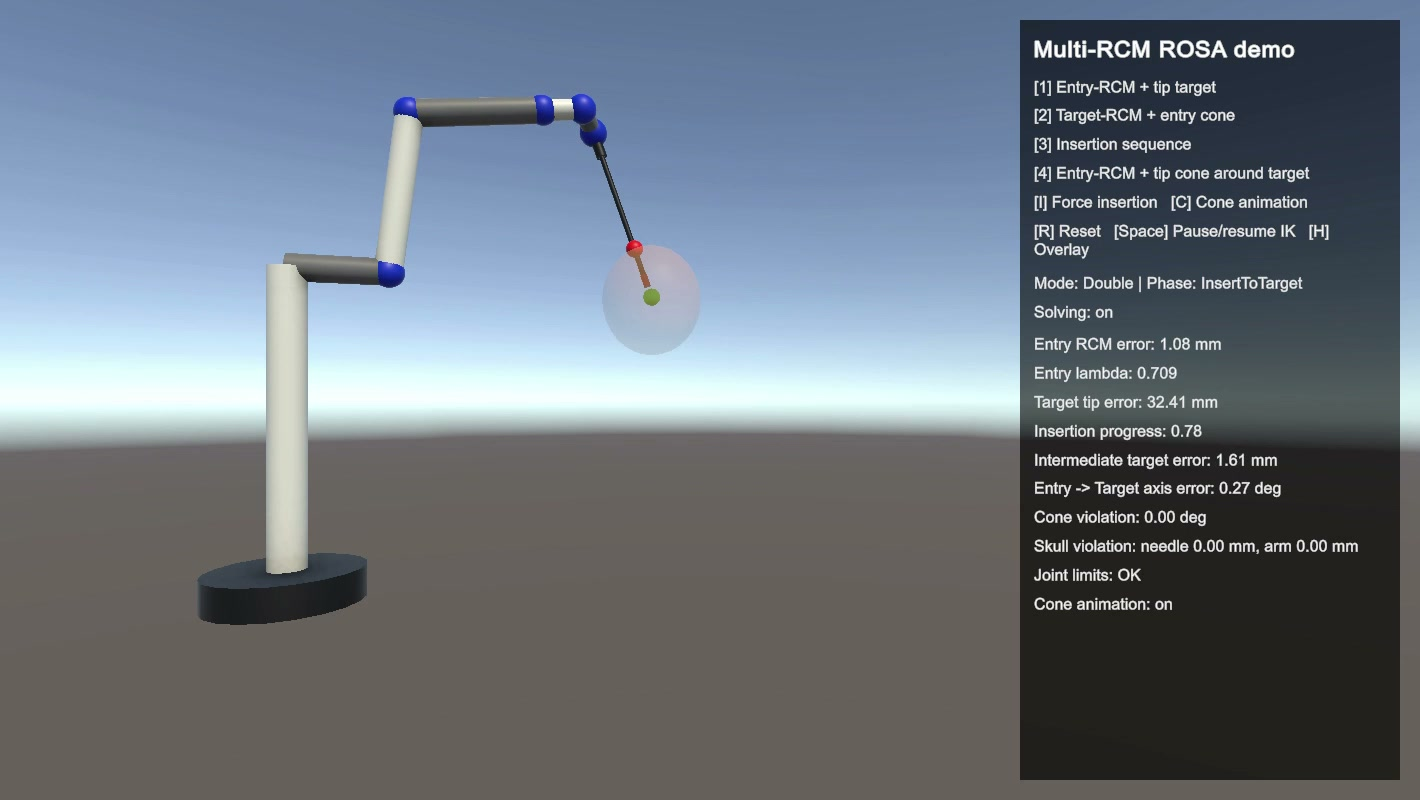
\includegraphics[width=0.55\textwidth]{unity_scene_wide.jpg}
\caption{Unity runtime overview: the 6R arm, needle shaft with tip/target markers, translucent skull sphere, and debug overlay. Illustrative screenshot; not tied to the numerical results of \cref{sec:results}.}
\label{fig:unity-scene}
\end{figure}

% =====================================================================
\section{Kinematic Control Framework}
\label{sec:kinematics}
% =====================================================================

\textbf{Forward kinematics and Jacobians.} Given $q\in\mathbb{R}^6$, forward kinematics is the standard product of DH transforms, $T_i(q)=T_{i-1}(q)A_i(q_i)$, giving the tool base point $p_{\mathrm{base}}(q)$ and axis $\hat z(q)$; any point at parameter $s\in[0,1]$ along the tool is $p_{\mathrm{tool}}(q,s)=p_{\mathrm{base}}(q)+sL\hat z(q)$, with the tip at $s=1$. \emph{Every} task-point Jacobian $J_i(q,\lambda)\in\mathbb{R}^{3\times7}$ -- tip, RCM point, cone points, insertion-axis guide point -- is computed by \emph{central finite differences} (perturbation $10^{-3}$ on each of the 7 extended-state components), not analytically, even where a closed form exists (e.g.\ $\partial p_{\mathrm{RCM}}/\partial\lambda=L\hat z(q)$).

\textbf{RCM geometry.} Following the reference paper's shaft-parameterization idea, the candidate RCM point slides along the fixed-length tool segment:
\begin{equation}
p_{\mathrm{RCM}}(q,\lambda) = p_{\mathrm{base}}(q) + \lambda\,L\,\hat z(q), \qquad \lambda\in[0.02,\,0.995].
\label{eq:rcm}
\end{equation}
$\lambda$ is stored as the seventh state component, integrated like a joint angle. A key structural difference from the reference: the ICRA paper enforces $p_{\mathrm{RCM}}\equiv p_{\mathrm{trocar}}$ as a \emph{hard} velocity constraint within the extended-task Jacobian; here ``RCM at entry'' (or ``at target'' in Task~2) is instead a \emph{soft, gain-weighted point-regulation task} stacked alongside the others, which can be transiently outweighed by competing tasks (\cref{sec:comparison,sec:discussion}).

\textbf{Task-space regulation and DLS solve.} Every controlled quantity is a 3-D point task $y_i=f_i(q,\lambda)$, $\dot y_i=J_i\dot x$. Each active task's error $e_i=y_{i,d}-y_i$ is magnitude-clipped and turned into a pure-proportional desired velocity $v_i=k_i\,\mathrm{sat}_{\varepsilon_i}(e_i)$ -- no feedforward term is ever added, even for the time-varying cone references of Tasks~2 and~4, which directly explains their non-zero steady-state tracking error (\cref{sec:results}). For all modes except Task~2's strict-priority solve, active tasks are stacked ($J=[J_1;\dots;J_m]$, $v=[v_1;\dots;v_m]$) and solved by damped least squares~\cite{nakamura1986}:
\begin{equation}
\dot x_{\mathrm{base}} = J^{\!\top}\left(JJ^{\!\top}+\mu^2 I\right)^{-1} v,
\label{eq:dls}
\end{equation}
plus an approximate null-space secondary term $\dot x = \dot x_{\mathrm{base}} + s_{\mathrm{ns}}\big(w - J^{\!\top}(JJ^{\!\top}+\mu_b^2 I)^{-1}(Jw)\big)$, where $w$ combines a joint-limit-avoidance gradient, a $\lambda$-regulation term toward a mode-dependent nominal $\lambda_d$, and a skull-avoidance gradient. The skull term is only active when \code{useSkullAvoidance} is true \emph{and} a skull exists; in the scene actually used, this flag is hard-coded \code{false}, so the term is inactive throughout the analysed run despite the skull sphere being present (\cref{sec:discussion}).

\textbf{Priority.} Tasks~1, 3, 4 use flat gain-weighted stacking (no exact hierarchy). Task~2 alone uses \emph{strict} task priority~\cite{siciliano1991}: the tip task is solved first, a tip null-space projector is built, and the entry-cone task is solved within it, with a final correction pass. Task~2 also implements an active-set guard on joint~4 (removes it from the stack if close to its limit); this guard never engaged in the analysed run.

\textbf{Singularity handling.} No SVD or condition number is computed. Instead, after each DLS solve the worst pre-saturation joint-speed ratio $\rho=\max_i|\dot x_i|/\dot q_{\max}$ ($\dot q_{\max}=\SI{80}{\degree\per\second}$) is checked; if $\rho>1$, the solve is repeated with boosted damping $\mu'=\mu\sqrt\rho\cdot1.2$. Hard saturation follows ($|\dot q_i|\le\SI{80}{\degree\per\second}$, $|\dot\lambda|\le\SI{0.55}{\per\second}$), then explicit-Euler integration sub-stepped at up to \SI{8}{\milli\second}, with joint/$\lambda$ clamping after every sub-step.

% =====================================================================
\section{Implemented Surgical Tasks}
\label{sec:tasks}
% =====================================================================

\begin{table}[H]
\centering\small
\caption{Point tasks stacked per mode (\code{BuildTasks()}). \checkmark marks the strict-priority solve.}
\label{tab:task-summary}
\begin{tabularx}{\textwidth}{c X c}
\toprule
Task & Point tasks (order = priority for T2 only) & Strict priority \\
\midrule
T1 -- Entry-RCM, tip target & tip$\to$target ($k=3.5$); RCM$\to$entry ($k=17.0$) & -- \\
T2 -- Target-RCM, entry cone & tip$\to$target ($k=3.5{\times}1.65$); entry-side$\to$cone ($k=6.0{\times}0.70$) & \checkmark \\
T3 -- Safe insertion & phase-dependent, see below & -- \\
T4 -- Entry-RCM, tip cone & tip$\to$cone ($k=3.5{\times}0.85$); RCM$\to$entry ($k=17.0{\times}1.6$) & -- \\
\bottomrule
\end{tabularx}
\end{table}

\textbf{Task~2 (target-centred RCM, entry cone).} The tip is the primary task, held at the deep target ($\lambda\to0.995$). The entry-side cone reference is $p_{\mathrm{cone},2}(t)=p_{\mathrm{entry}}+r_2(\cos\phi\,\hat b_1+\sin\phi\,\hat b_2)$, $r_2=d_{\mathrm{ET}}\tan\theta_c\approx\SI{8.79}{\milli\meter}$ ($d_{\mathrm{ET}}=\SI{111.7}{\milli\meter}$, $\theta_c=4.5^{\circ}$), $\phi(t)=\omega_2 t^+$, $\omega_2=\SI{8}{\degree\per\second}$ (deliberately lowered from an earlier \SI{12}{\degree\per\second} to keep tip-target error under threshold). An explicit \code{RCMPoint}$\to$\code{target} task was removed from the stack (duplicated the tip task, caused jitter); \code{target\_rcm\_error\_mm} is therefore a diagnostic, not an actively minimized quantity.

\textbf{Task~3 (safe insertion).} A finite-state machine with phases \code{ApproachEntry} (tip $\to$ pre-entry point \SI{10}{\centi\meter} outside the body; no RCM task), \code{PierceEntry} (tip interpolates to the entry point; soft RCM pre-stabilization added past 80\% progress; $\lambda$ force-set to 0.995 on exit), \code{InsertToTarget} (RCM task active with boosted gain $\times1.6$, tip gain reduced $\times0.85$, favouring pivot stability over insertion speed), and \code{Done} (holds the final pose). A continuous secondary ``insertion-axis guide point'' task runs throughout all three active phases to keep the shaft collinear with the entry-target line.

\textbf{Task~4 (entry-centred RCM, tip cone).} The entry-RCM task stays active (gain $\times1.6$) while the tip traces a cone of fixed radius $r_4=\SI{13.8}{\milli\meter}$ around the target, $p_{\mathrm{cone},4}(t)=p_{\mathrm{target}}+r_4(\cos\phi\,\hat b_1+\sin\phi\,\hat b_2)$, $\omega_4=\SI{7}{\degree\per\second}$ (slower than Task~2's $\omega_2$, and null-space scale reduced $\times0.35$) so the RCM task wins the flat-weighted conflict with the moving cone reference.

Transitions between Tasks~1--4 are operator-triggered keyboard events; only the internal Task-3 phase transitions are autonomous. Every mode switch has a shared \SI{1.5}{\second} cone warm-up delay before the cone phase angle begins to sweep.

% =====================================================================
\section{Experimental Methodology}
\label{sec:methodology}
% =====================================================================

All quantitative results come exclusively from \texttt{RCM\_logs/\allowbreak project4\_\allowbreak multircm\_\allowbreak 20260714\_\allowbreak 193548\_422.csv} (2696 samples, \SI{157.258}{\second}), one continuous session visiting modes \code{3}$\to$\code{1}$\to$\code{2}$\to$\code{4} with no restarts. The \code{RCM\_logs/} directory contains 21 other logs from the same session; none were used for any statistic in this report. Segmentation (\cref{tab:segments}) was derived directly from the CSV's \code{task}/\code{phase} columns.

\begin{table}[H]
\centering\small
\caption{Pipeline segmentation from the selected CSV. $n$: sample count.}
\label{tab:segments}
\begin{tabular}{l S[table-format=3.2] r}
\toprule
Task/Phase & {Duration [s]} & $n$ \\
\midrule
T3 -- ApproachEntry & 1.03 & 19 \\
T3 -- PierceEntry & 6.21 & 117 \\
T3 -- InsertToTarget & 9.96 & 180 \\
T3 -- Done & 9.33 & 174 \\
T1 -- Entry-RCM, tip target & 3.94 & 71 \\
T2 -- Target-RCM, entry cone & 64.37 & 1097 \\
T4 -- Entry-RCM, tip cone & 61.99 & 1038 \\
\bottomrule
\end{tabular}
\end{table}

Two thresholds come directly from the controller's public fields (echoed in the CSV header): \code{entryRcmOkThresholdMm}~$=\SI{2.0}{\milli\meter}$ and \code{tipTargetOkThresholdMm}~$=\SI{3.0}{\milli\meter}$, approximating clinical stereotactic accuracy. The skull threshold is \SI{0}{\milli\meter}. A \SI{50}{\milli\meter}$\;$cone-tracking reference line is used only as a loose sanity-check, not a pass/fail criterion. Following the analyzer's convention, entry-RCM and tip-target statistics exclude the first \SI{1}{\second} after each switch (``settled'' window); the full-phase (transient-inclusive) maximum is always reported alongside it.

% =====================================================================
\section{Results}
\label{sec:results}
% =====================================================================

\begin{figure}[H]
\centering

\includegraphics[width=0.72\textwidth]{00_task_timeline.png}
\caption{Executed task timeline, whole run ($t\in[0,157.3]\,\mathrm{s}$). Steps mark manually triggered mode switches; no automatic supervisor chains the tasks.}
\label{fig:timeline}
\end{figure}

\FloatBarrier
\subsection{Task 2 -- Target-Centred RCM, Entry Cone}
\label{sec:results-t2}

Over the full \SI{64.37}{\second} segment ($n=1097$), the entry-cone tracking error had mean \SI{4.96}{\milli\meter}, RMS \SI{6.13}{\milli\meter}, median \SI{4.17}{\milli\meter}, 95th percentile \SI{13.17}{\milli\meter}, max \SI{13.67}{\milli\meter} against a commanded radius $r_2\approx\SI{8.79}{\milli\meter}$ -- comparable in magnitude to the radius itself (\cref{fig:t2-cone}). The tip-target error (primary task) had mean only \SI{0.006}{\milli\meter}, max \SI{0.26}{\milli\meter}, confirming the tip stays essentially frozen at the target while the cone task absorbs the tracking lag. The diagnostic \code{target\_rcm\_error\_mm} remained near-constant at \SI{1.42}{\milli\meter} (std \SI{0.003}{\milli\meter}), consistent with a static geometric offset rather than an actively minimized quantity.

\begin{figure}[H]
\centering

\includegraphics[width=0.6\textwidth]{04_T2_entry_cone_error.png}
\caption{Task~2, entry-cone tracking error (mm) vs.\ local task time, full \SI{64.37}{\second} segment. Dashed line: \SI{50}{\milli\meter} sanity-check reference (not a threshold); commanded cone radius itself is $\approx\SI{8.79}{\milli\meter}$.}
\label{fig:t2-cone}
\end{figure}

\FloatBarrier
\subsection{Task 3 -- Safe Insertion}
\label{sec:results-t3}

During \code{InsertToTarget} ($n=180$ full / $160$ settled), entry-RCM error reached a full-phase max of \SI{4.84}{\milli\meter} (mode-switch transient) but, settled, had mean \SI{0.179}{\milli\meter}, RMS \SI{0.188}{\milli\meter}, max \SI{0.237}{\milli\meter} -- well inside the \SI{2}{\milli\meter} threshold. During \code{Done} ($n=174$ full / $155$ settled), it settled further to mean \SI{0.091}{\milli\meter}, max \SI{0.151}{\milli\meter}. The final tip-to-target error (last logged sample) was \SI{0.467}{\milli\meter} (settled-window mean \SI{0.752}{\milli\meter}, max \SI{1.498}{\milli\meter}), inside the \SI{3}{\milli\meter} threshold. \code{skull\_violation\_mm} was identically zero across all 490 Task-3 samples; \cref{sec:discussion} explains why this alone is not evidence of collision safety. Tool-axis angular error had median \SI{1.08}{\degree} over \code{InsertToTarget}+\code{Done}, dropping to \SI{0.27}{\degree} at the final sample.

\begin{figure}[H]
\centering
\begin{subfigure}{0.49\textwidth}

\includegraphics[width=\textwidth]{02_T3_entry_rcm_error.png}
\caption{Entry-RCM error, \code{InsertToTarget}+\code{Done}.}
\label{fig:t3-entry-rcm}
\end{subfigure}\hfill
\begin{subfigure}{0.49\textwidth}

\includegraphics[width=\textwidth]{02b_T3_tip_target_error.png}
\caption{Final tip-to-target error, \code{Done} phase.}
\label{fig:t3-tip-target}
\end{subfigure}
\caption{Task~3, safe insertion. (a) Entry-RCM error (mm), threshold \SI{2}{\milli\meter}: settled max \SI{0.237}{\milli\meter}. (b) Tip-to-target error (mm), threshold \SI{3}{\milli\meter}: final value \SI{0.467}{\milli\meter}.}
\label{fig:t3-pair}
\end{figure}

\FloatBarrier
\subsection{Task 4 -- Entry-Centred RCM, Tip Cone}
\label{sec:results-t4}

Over the full \SI{61.99}{\second} segment ($n=1038$), settled entry-RCM error ($n=1021$) had mean \SI{0.353}{\milli\meter}, RMS \SI{0.425}{\milli\meter}, max \SI{0.834}{\milli\meter} (inside the \SI{2}{\milli\meter} threshold), while the full-phase max was \SI{3.84}{\milli\meter} (mode-switch transient). The tip-cone tracking error had settled mean \SI{3.19}{\milli\meter}, RMS \SI{3.67}{\milli\meter}, max \SI{7.11}{\milli\meter} against the commanded $r_4=\SI{13.8}{\milli\meter}$ radius -- tighter, relative to the commanded radius, than Task~2's entry-cone tracking, consistent with the reduced cone speed and gain rebalancing of \cref{sec:tasks}.

\begin{figure}[H]
\centering
\begin{subfigure}{0.49\textwidth}

\includegraphics[width=\textwidth]{06_T4_entry_rcm_error.png}
\caption{Entry-RCM error.}
\label{fig:t4-entry-rcm}
\end{subfigure}\hfill
\begin{subfigure}{0.49\textwidth}

\includegraphics[width=\textwidth]{07_T4_tip_cone_error.png}
\caption{Tip-cone tracking error.}
\label{fig:t4-tip-cone}
\end{subfigure}
\caption{Task~4, full \SI{61.99}{\second} segment. (a) Entry-RCM error (mm): settled max \SI{0.834}{\milli\meter}, transient max \SI{3.84}{\milli\meter}. (b) Tip-cone tracking error (mm) against $r_4=\SI{13.8}{\milli\meter}$: settled mean \SI{3.19}{\milli\meter}, max \SI{7.11}{\milli\meter}.}
\label{fig:t4-pair}
\end{figure}

\FloatBarrier
\subsection{Velocity and Runtime Diagnostics}
\label{sec:results-diag}

Across the whole run, commanded joint-velocity norm $\lVert\dot q\rVert$ had mean \SI{0.063}{\radian/\second} and max \SI{1.25}{\radian/\second}, approaching but not reaching the \SI{80}{\degree\per\second}$\approx\SI{1.396}{\radian/\second}$ per-joint saturation limit. $\lambda$ ranged from $0.601$ to $0.995$. Editor frame rate ranged \SIrange{5.8}{213.0}{\hertz} (mean \SI{58.4}{\hertz}) -- an editor/host-load artifact, not a real-time guarantee. Jacobian-conditioning diagnostics (condition number, $\sigma_{\min}$) are implemented in the analyzer but not produced here, as the required columns are absent from the current CSV logger.

\FloatBarrier
\subsection{Summary Table}
\label{sec:results-table}

\begin{table}[H]
\centering\small
\caption{Selected rows of the full metrics table (\texttt{report/final\_metrics\_table.csv}, 29 rows). ``Settled'' excludes the first \SI{1}{\second} after each switch; ``--'' = not pass/fail-gated.}
\label{tab:summary}
\begin{tabularx}{\textwidth}{X l S[table-format=2.3] S[table-format=2.3] c c}
\toprule
Task / phase / metric & Unit & {Mean} & {Max} & Thr. & Result \\
\midrule
T3 InsertToTarget (settled) entry-RCM error & mm & 0.179 & 0.237 & 2.0 & \pass \\
T3 Done (settled) entry-RCM error & mm & 0.091 & 0.151 & 2.0 & \pass \\
T3 Done (settled) tip-target error & mm & 0.752 & 1.498 & 3.0 & \pass \\
T3 all phases skull violation & mm & 0.000 & 0.000 & 0.0 & \pass$^{\ast}$ \\
T2 entry-cone tracking error (full) & mm & 4.956 & 13.665 & -- & -- \\
T2 tip-target error (settled) & mm & 0.005 & 0.009 & 3.0 & \pass \\
T4 entry-RCM error (settled) & mm & 0.353 & 0.834 & 2.0 & \pass \\
T4 tip-cone tracking error (settled) & mm & 3.194 & 7.109 & -- & -- \\
T1 entry-RCM error (brief, transient-dominated) & mm & 0.076 & 0.088 & -- & -- \\
\bottomrule
\end{tabularx}
\vspace{2pt}
\footnotesize $^{\ast}$Skull avoidance is inactive in this run and the corridor is exempted from the check by construction; PASS reflects the logged value, not a validated collision-safety guarantee (\cref{sec:discussion}).
\end{table}

% =====================================================================
\section{Comparison with the ICRA 2013 RCM Approach}
\label{sec:comparison}
% =====================================================================

\begin{table}[H]
\centering
\footnotesize
\caption{Aspect-by-aspect comparison between Aghakhani et al.\ (ICRA 2013)~\cite{aghakhani2013} and this project.}
\label{tab:comparison}
\begin{tabularx}{\textwidth}{l X X}
\toprule
Aspect & ICRA 2013 paper & This project \\
\midrule
Application & Endoscopic-camera visual servoing; obstacle-avoiding path following & Needle/electrode positioning for stereotactic neurosurgery \\
Robot platform & KUKA KR5 (Webots); DLR MIRO & Procedural ROSA-like 6R arm (Unity, no physics engine) \\
RCM definition & Slides along segment between two DH frame origins & Slides along the fixed-length rigid-tool segment (same idea) \\
RCM location & Fixed at entry/trocar & Entry-centred (T1/3/4) \emph{and} target-centred (T2) \\
Task combination & RCM as hard velocity constraint in one extended Jacobian & RCM as a soft, gain-weighted task, flat (T1/3/4) or strict-priority (T2 only) \\
Jacobian & Analytic & Purely numerical, central finite differences \\
Singularity handling & Not addressed explicitly & Adaptive damping triggered by a joint-speed-saturation proxy \\
Joint limits & Not modelled & Hard DH clamp + soft null-space term + T2-only joint-4 guard \\
Safety modelling & RCM only (+ null-space obstacle avoidance in 9-DOF example) & Skull-avoidance term implemented but disabled; always-on diagnostic with corridor exemption \\
Validation & Simulation only, single/few runs & Simulation only, one continuous run across all four modes \\
Main limitation & No hardware validation; no joint-limit/singularity treatment & Kinematic-only; RCM is soft, so transiently violated at mode switches \\
\bottomrule
\end{tabularx}
\end{table}

The paper's classical entry-port RCM corresponds directly to this project's entry-centred mode (T1/3/4); the target-centred mode (T2) has no direct counterpart and is an untested extension of the same segment-parameterization idea with the roles of fixed/moving point swapped. Switching between RCM placements here is realized purely by changing which point tasks are stacked, exploiting a task-agnostic finite-difference Jacobian pipeline -- the paper does not consider switchable RCM placements. Both works track moving references (conical/path-following) with pure proportional feedback and no explicit feedforward, so the steady-state cone-tracking lag reported in \cref{sec:results-t2,sec:results-t4} is a direct, expected consequence of that shared choice, not an implementation defect. The paper's Jacobians are analytic with undetailed damping/singularity handling; this project trades that rigor for a fully numerical pipeline plus an explicit adaptive-damping trigger, at a small constant per-step cost. Neither work presents hardware validation, and no cross-comparison of absolute accuracy is claimed given the differing platforms and scope.

\subsection{Why These Choices Were Made}
\label{sec:comparison-rationale}

None of the deviations from the reference formulation are arbitrary: each follows from a concrete requirement of this project that the paper's two worked examples did not have to satisfy.

\begin{description}[leftmargin=0pt,style=nextline]
\item[\textbf{Soft, gain-weighted RCM task instead of a hard velocity constraint.}] The paper enforces one fixed RCM placement per experiment, so a single dedicated extended-Jacobian block is sufficient. This project instead needed \emph{four} modes sharing one controller -- entry-centred, target-centred, a phased insertion, and a cone motion -- switched live by the operator. Treating the RCM condition as one more point task, with its own gain, lets \code{BuildTasks()} assemble any mode by simply choosing which points to stack and with what weight, without a different Jacobian-block structure per mode. The cost, an RCM that can be transiently outweighed by a competing task, was accepted because the settled-state results (\cref{sec:results}) show it converges to sub-millimetre accuracy in practice for the tuned gains used here.
\item[\textbf{Purely numerical (finite-difference) Jacobians instead of analytic ones.}] This project has many more distinct task points than the paper's examples (tip, entry-RCM, target-RCM, two different cone points, an insertion-axis guide point), each only active in some modes/phases. Deriving and maintaining a correct analytic Jacobian for every point, and keeping all of them consistent whenever the DH table or a task-point definition changed during development, was judged more error-prone and slower to iterate on than one generic central-difference routine that is automatically correct for any point defined through the same forward-kinematics chain. The trade is a small, constant extra cost (7 extra forward-kinematics evaluations per solve) against a much smaller surface for bugs.
\item[\textbf{Strict task priority only for Task~2, flat weighting elsewhere.}] Task~2 is the one mode where the tip \emph{must} stay essentially motionless at the deep target while a secondary motion happens at the entry side -- exactly the situation exact priority is designed for, since it guarantees the lower-priority cone task cannot leak into the tip's accuracy. Tasks~1, 3, and~4 do not have this same asymmetric criticality (their competing tasks are both required to converge, not one frozen and one moving), so the extra implementation cost of a strict-priority solve -- a dedicated null-space projector, a correction pass, and its own singularity re-solve -- was reserved for the one case that actually needed it, and gain tuning was used to manage the RCM/tip trade-off in the other three.
\item[\textbf{Heuristic adaptive damping instead of an SVD/condition-number-based singularity index.}] Every DLS solve in this project already runs inside a per-frame loop that can be sub-stepped up to 8 times (\cref{sec:kinematics}), and every sub-step already pays for a full finite-difference Jacobian rebuild. Adding a singular-value decomposition on top of that, potentially several times per rendered frame, was judged an unnecessary real-time cost when a much cheaper proxy -- the worst pre-saturation joint-speed ratio -- flags the same near-singular configurations (a joint being asked to move faster than it can) in time to boost damping before saturation clips the command.
\item[\textbf{A target-centred RCM mode (Task~2) not present in the paper.}] The paper only demonstrates the entry-port RCM. Once the controller represents the RCM point as $p_{\mathrm{base}}(q)+\lambda L\hat z(q)$, nothing in the geometry actually requires $\lambda$ to be driven toward the entry side: driving it toward $\lambda\approx1$ instead relocates the same machinery's practical role to the target. This was added because it models a clinically plausible complementary scenario -- the tip already at the target while a small, controlled motion is still needed at the skin/entry side -- using the identical $\lambda$-based formalism, rather than a second, unrelated control law.
\item[\textbf{A three-phase insertion state machine instead of the four-phase one originally planned.}] A separate \code{AlignAtEntry} phase was planned to align the shaft with the entry-target line before insertion, but was dropped in favour of a continuous secondary ``insertion-axis guide point'' task that runs throughout \code{ApproachEntry}, \code{PierceEntry}, and \code{InsertToTarget}. Gating alignment behind its own phase would have added another transition condition (and another transient at that boundary) for a behaviour that a continuously active secondary task already achieves smoothly.
\item[\textbf{Hard joint limits, null-space avoidance, and a Task-2-only joint-4 guard, none of which the paper models.}] The paper's visual-servoing and motion-planning examples do not report joint-limit handling. This project's insertion task, by contrast, sweeps the arm between a pose \SI{10}{\centi\meter} outside the body and a deep insertion pose, a much larger excursion where hitting a joint limit is a real risk; hard clamping plus a soft null-space avoidance term were added specifically to keep that excursion feasible, and the joint-4 active-set guard was added only for Task~2 because that is the one mode whose strict-priority solve was, during development, observed to occasionally drive joint~4 toward its limit.
\item[\textbf{Manually tuned, mode-specific gain multipliers instead of a single global gain set or a systematic optimization.}] Several multipliers (e.g.\ Task~2's cone-speed reduction from \SI{12}{\degree\per\second} to \SI{8}{\degree\per\second}, documented in the code's own comments) were adjusted iteratively in direct response to a specific observed failure mode -- in that case, the tip-target error exceeding the \SI{3}{\milli\meter} threshold at the faster cone speed. Given the project's simulation-only, single-scenario scope, this iterative approach was judged sufficient to satisfy the clinically motivated thresholds for the analysed geometry, at the acknowledged cost of not generalizing automatically to a different entry/target configuration (\cref{sec:discussion}).
\end{description}

% =====================================================================
\section{Discussion, Limitations, and Future Work}
\label{sec:discussion}
% =====================================================================

\textbf{Precision and transients.} Once settled, entry-RCM error stayed below \SI{0.9}{\milli\meter} in every regulated task, an order of magnitude inside the \SI{2}{\milli\meter} threshold, and the final insertion error (\SI{0.467}{\milli\meter}) is well inside \SI{3}{\milli\meter} -- for this geometry and gain set, the soft-task RCM formulation behaves close to a hard constraint, though this is an emergent, tuned-gain property, not a structural guarantee. Every mode switch produces a transient spike in the newly regulated error (\SI{4.84}{\milli\meter} at \code{PierceEntry}$\to$\code{InsertToTarget}, \SI{3.84}{\milli\meter} at T2$\to$T4), decaying within \SI{1}{\second}: a single continuous run captures real transient behaviour that a steady-state-only summary would hide.

\textbf{RCM-vs-cone trade-off.} Tasks~2 and~4 both couple a fixed-point task with a moving cone reference; the code's gain multipliers are direct evidence of hand-tuning this trade-off (T2: cone gain $\times0.70$, tip gain $\times1.65$; T4: tip-cone gain $\times0.85$, RCM gain $\times1.6$). The measured cone errors (T2 mean \SI{4.96}{\milli\meter}/\SI{8.79}{\milli\meter} radius; T4 mean \SI{3.19}{\milli\meter}/\SI{13.8}{\milli\meter} radius) show the trade-off is real: the pure-proportional law has no feedforward to compensate a continuously moving reference, and protecting the higher-priority task necessarily slows the lower-priority one further.

\textbf{Single-run caveat.} Every number in \cref{sec:results} comes from one continuous, operator-paced run; sample counts are large (up to 1097 for T2) but temporally correlated, not independent trials. Results should be read as ``this run satisfied these thresholds,'' not a validated success rate across conditions.

\textbf{Key limitations.}
\begin{itemize}[leftmargin=14pt]
\item Purely kinematic: no dynamics, actuator bandwidth, or force/torque control; velocities are integrated directly into positions.
\item No tissue interaction/deformation; the skull is a rigid static sphere for a soft cost/violation check only, no physical trocar model.
\item Skull avoidance is implemented but hard-coded \code{false} at scene-build time; the always-zero \code{skull\_violation\_mm} reading reflects avoidance being off and a corridor exemption that structurally excludes on-axis motion -- \emph{not} evidence of collision safety.
\item No sensor noise, calibration error, or communication delay anywhere in the loop.
\item All Jacobians are finite-difference, not analytic, even where closed forms exist.
\item Gains are manually tuned per mode, not systematically optimized; integration is explicit Euler, sub-stepped but not adaptive.
\item Single selected run, no repeated trials or statistical evaluation; DH table is plausible, not the real manufacturer's; no hardware or clinical validation.
\end{itemize}

\textbf{Future work.} Hardware or higher-fidelity physics validation with real DH parameters; ROS/ROS~2 integration; torque-level dynamics-aware control; tissue-interaction/force feedback replacing the static skull sphere; an active always-on collision-avoidance term; formulating RCM and joint/velocity limits as hard constraints in a QP rather than soft tasks; a consistent hierarchical priority scheme across all four modes; principled/optimized gain tuning; robustness studies (noise, registration error, latency); repeated trials across postures and geometries with proper statistics; and a controlled comparison against a hard-constraint or QP-based virtual-fixture RCM controller.

% =====================================================================
\section{Conclusion}
\label{sec:conclusion}
% =====================================================================

This report reconstructed, from the C\# source of a from-scratch Unity controller, a purely kinematic, penetration-coordinate RCM scheme in the spirit of Aghakhani et al.\ (ICRA 2013), implementing entry-centred and target-centred RCM modes, a three-phase safe-insertion sequence, and an entry-centred conical tip motion. Every quantitative claim was computed from one selected experimental log and independently re-verified. Within that run, all settled entry-RCM and tip-target statistics satisfy the \SI{2}{\milli\meter}/\SI{3}{\milli\meter} clinical thresholds, while the conical-motion tracking errors in Tasks~2 and~4 reveal a real, gain-tunable trade-off between pivot stability and moving-reference tracking under pure proportional control. The comparison with the reference paper shows a project that trades the paper's analytic, hard-constraint RCM formulation for a more flexible, purely numerical, multi-mode, soft-task architecture -- a reasonable engineering trade-off for a simulation-only, exploratory implementation, not a claim of improving on the reference method.

% =====================================================================
\appendix
\section{Controller Parameters and Reproducibility}
\label{app:params}
% =====================================================================

\begin{table}[H]
\centering\small
\caption{Key controller gains and thresholds as coded (Inspector defaults).}
\label{tab:gains}
\begin{tabular}{l l | l l}
\toprule
Parameter & Value & Parameter & Value \\
\midrule
Base tip / RCM / cone gain & 3.5 / 17.0 / 6.0 & T2 tip/cone/damp/ns mult. & $\times$1.65/0.70/1.0/0.6 \\
Base damping $\mu_0$ & 0.055 & T4 tip/RCM/damp/ns mult. & $\times$0.85/1.6/0.7/0.35 \\
Max joint speed / $\dot\lambda$ & \SI{80}{\degree\per\second} / \SI{0.55}{\per\second} & Cone half-angle $\theta_c$ & \SI{4.5}{\degree} \\
Singularity trigger / boost & 1.0 / 1.2 & Cone speed $\omega_2$/$\omega_4$ & \SI{8}{}/\SI{7}{\degree\per\second} \\
Entry-RCM / tip-target thr. & \SI{2.0}{}/\SI{3.0}{\milli\meter} & Task-4 cone radius $r_4$ & \SI{13.8}{\milli\meter} \\
\bottomrule
\end{tabular}
\end{table}

\textbf{Reproducibility.} Source log: \texttt{RCM\_logs/\allowbreak project4\_\allowbreak multircm\_\allowbreak 20260714\_\allowbreak 193548\_422.csv} (fixed, not glob-selected). Pipeline: \texttt{.venv/\allowbreak bin/\allowbreak python3 report/\allowbreak scripts/\allowbreak generate\_\allowbreak final\_\allowbreak run\_\allowbreak metrics.py} calls the unmodified \code{analyze\_\allowbreak rcm\_\allowbreak logs\_\allowbreak clean.py} on this file, writing figures to \code{report/\allowbreak generated\_\allowbreak figures/} and \code{final\_\allowbreak metrics\_\allowbreak table.csv}; then \texttt{cd report \&\& tectonic report.tex} compiles this document. Full details, including the ten-value independent numerical-verification pass, are recorded in \texttt{report/\allowbreak REPORT\_\allowbreak GENERATION\_\allowbreak NOTES.md}.

% =====================================================================
\begin{thebibliography}{9}

\bibitem{aghakhani2013}
N.~Aghakhani, M.~Geravand, N.~Shahriari, M.~Vendittelli, G.~Oriolo,
``Task Control with Remote Center of Motion Constraint for Minimally Invasive Robotic Surgery,''
\emph{2013 IEEE International Conference on Robotics and Automation (ICRA)}, Karlsruhe, Germany, May 6--10, 2013, pp.~5807--5812.

\bibitem{nakamura1986}
Y.~Nakamura, H.~Hanafusa,
``Inverse Kinematic Solutions with Singularity Robustness for Robot Manipulator Control,''
\emph{ASME Journal of Dynamic Systems, Measurement, and Control}, vol.~108, 1986.

\bibitem{siciliano1991}
B.~Siciliano, J.-J.~E.~Slotine,
``A General Framework for Managing Multiple Tasks in Highly Redundant Robotic Systems,''
in \emph{Proc.\ 5th Int.\ Conf.\ on Advanced Robotics (ICAR)}, 1991, pp.~1211--1216.

\end{thebibliography}

\end{document}
